\subsection{Analisi dei compiti e degli scenari}

In questa sezione vengono analizzati nel dettaglio i singoli compiti e gli scenari dell'esperimento con gli utenti. Ciascun compito viene valutato sia a livello generale, sia dividendo i dati in base all'ordine di esecuzione (A-B e B-A) per osservare l'eventuale effetto di apprendimento.

Nella valutazione dei risultati, è stata data maggiore importanza alla riduzione degli errori e all'accuratezza dell'interazione rispetto al puro tempo di completamento. Di conseguenza, un leggero aumento dei tempi nella versione riprogettata viene considerato un compromesso accettabile per garantire una procedura più fluida, chiara e priva di blocchi per l'utente.

\subsubsection{Compito C1: Registrazione e inserimento dati accademici}
Il compito C1 prevedeva il completamento della procedura di registrazione alla piattaforma, comprensiva dell'inserimento delle credenziali di accesso e dei dati accademici (Università, Dipartimento e Corso di studi). L'obiettivo di questo compito era valutare l'usabilità del form di registrazione, verificando l'effettiva riduzione degli errori sistematici riscontrati nella versione originale attraverso l'introduzione di un form multi-step guidato (wizard) nella versione riprogettata.

\paragraph{Analisi delle prestazioni generali}
Come si evince dalla Tabella~\ref{tab:6-c1-1}, il tasso di completamento (Success Rate) si è attestato al 100\% per entrambe le versioni del sistema. I dati rilevano un abbattimento dell'80,00\% nella media degli errori e una contrazione della mediana dei click (-15,79\%) a favore della versione riprogettata. Di contro, si osserva un incremento del 14,29\% nella mediana del tempo di esecuzione per la versione B.

\begin{table}[H]
	\centering
	\small
	\renewcommand{\arraystretch}{1.2}
	\caption{Metriche prestazionali globali aggregate per il compito C1.}
	\label{tab:6-c1-1}
	\begin{tabular}{|l|c|c|c|}
		\hline
		\rowcolor{gray!30}
		\textbf{Metrica} & \textbf{Versione originale (A)} & \textbf{Versione post-riprogettazione (B)} & \textbf{Variazione} \\ \hline
		Success Rate     & 100,00\%                        & 100,00\%                                   & 0,00\%              \\ \hline
		Media Errori     & 1,00                            & 0,20                                       & -80,00\%            \\ \hline
		Mediana Tempo    & 1:10.00                         & 1:20.00                                    & 14,29\%             \\ \hline
		Mediana Click    & 19                              & 16                                         & -15,79\%            \\ \hline
		Media Difficoltà & 1,33                            & 1,20                                       & -10,00\%            \\ \hline
	\end{tabular}
\end{table}

La significativa riduzione del numero medio di errori e di click complessivi trova giustificazione nella riorganizzazione strutturale dell'interfaccia di input. L'introduzione della validazione contestuale e di indicatori chiari di avanzamento ha permesso di prevenire gli errori di inserimento tipici della versione originale. L'aumento del tempo mediano di completamento nella versione riprogettata è direttamente riconducibile alla nuova struttura a step e all'inserimento di una schermata di riepilogo finale. Tale scelta progettuale privilegia deliberatamente l'accuratezza dei dati inseriti rispetto alla rapidità di esecuzione, aumentando le probabilità di esiti positivi durante la compilazione del form e limitando la necessità di correzioni successive.

\paragraph{Analisi qualitativa: commenti e osservazioni degli utenti}

I dati quantitativi trovano un forte riscontro qualitativo nelle annotazioni degli sperimentatori e nei commenti espliciti rilasciati dagli utenti durante il test (\textit{thinking aloud}).

Per la versione originale (A), sono emerse diverse criticità ricorrenti:

\begin{itemize}
	\item \textbf{Coerenza linguistica}: molti utenti hanno lamentato la presenza della lingua inglese nel form di registrazione. Questo ha generato confusione sul significato di alcuni pulsanti. Tale problematica rappresenta una netta violazione del principio di coerenza linguistica con il resto della piattaforma in italiano.

	\item \textbf{Effetto ``Flash'' e distrazione}: diversi partecipanti hanno segnalato un forte fastidio causato da un ``effetto flash'' (la schermata diventava completamente bianca per qualche milli-secondo) durante la compilazione. Questo bug visivo si è rivelato un grave elemento di distrazione: in più occasioni ha indotto l'utente a dimenticare di selezionare campi obbligatori (come il corso di studio). La situazione è stata aggravata dalla totale assenza di messaggi di errore chiari e tempestivi al momento del salvataggio.

	\item \textbf{Mancanza di visibilità dello stato}: è emersa un'esplicita frustrazione legata all'impossibilità di visualizzare in chiaro la password digitata. Questa criticità giustifica pienamente l'implementazione del pattern \textit{Password Strength Meter} (con l'apposito \textit{toggle} per la visibilità) introdotto nella versione B.

	\item \textbf{Navigazione iniziale}: il flusso per raggiungere il form di registrazione dalla homepage è stato giudicato a tratti poco intuitivo, con alcuni utenti che si aspettavano opzioni esplicite come ``non ho un account'' direttamente nella schermata di login.
\end{itemize}

Passando alla versione post-riprogettazione (B), le considerazioni generali sono mutate radicalmente in positivo, confermando il successo delle scelte di design adottate:

\begin{itemize}
	\item \textbf{Apprezzamento per il Riepilogo}: la novità più elogiata in assoluto è stata l'introduzione dello step finale, rinominato in ``Riepilogo'' (invece del generico ``Fatto''). Molti utenti hanno esplicitamente apprezzato questa schermata. L'apprezzamento deriva dal fatto che ha restituito loro il controllo sui dati accademici prima della conferma finale.

	\item \textbf{Linearità del flusso}: l'approccio strutturato in step progressivi ha reso il compito percepito come ``più lineare''.

	\item \textbf{Innalzamento delle aspettative}: l'impatto dei miglioramenti è perfettamente sintetizzato dal commento di un utente (sottoposto all'ordine B-A) che, dopo aver completato il compito sulla nuova interfaccia, ha ammesso: ``Se avessi visto questo prima, sarei stato più cattivo con la versione A''. Ciò dimostra come il nuovo design abbia innalzato le aspettative di usabilità, rendendo evidenti e intollerabili i difetti della versione precedente.
\end{itemize}

\paragraph{Valutazione dell'effetto di apprendimento}
Analizzando i dati in base all'ordine di esecuzione, emergono variazioni significative nei tempi di completamento. Per il gruppo sottoposto all'ordine A-B, si osserva un tempo mediano maggiore nella versione originale, che si riduce notevolmente durante l'utilizzo della versione B. Nel gruppo associato all'ordine B-A, l'esperienza pregressa maturata sulla versione riprogettata ha abbattuto il tempo necessario per completare il medesimo compito sulla versione originale. Questo risultato evidenzia un trasferimento positivo della conoscenza delle operazioni richieste, che ha parzialmente compensato i limiti strutturali e la mancanza di feedback della variante originale.

\begin{figure}[H]
	\centering
	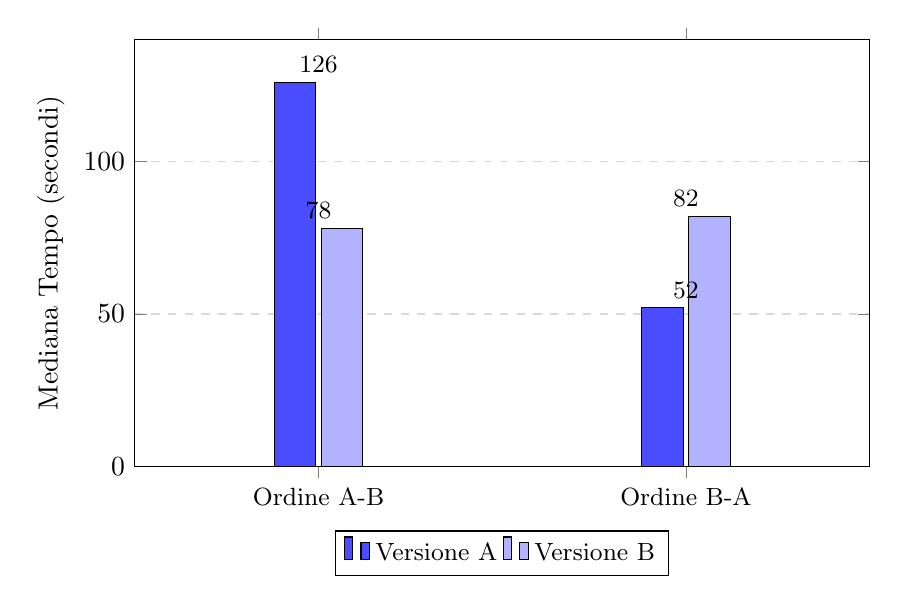
\begin{tikzpicture}
		\begin{axis}[
				ybar,
				bar width=15pt,
				width=0.9\textwidth,
				height=7cm,
				symbolic x coords={Ordine A-B, Ordine B-A},
				xtick=data,
				x tick label style={font=\small},
				ylabel={Mediana Tempo (secondi)},
				ymin=0, ymax=140,
				ymajorgrids=true,
				grid style={dashed, gray!30},
				enlarge x limits=0.5,
				legend style={at={(0.5,-0.15)}, anchor=north, legend columns=-1, font=\small},
				nodes near coords,
				every node near coord/.style={font=\small, color=black},
			]
			\addplot+[ybar, fill=blue!70, draw=black] coordinates {(Ordine A-B,126) (Ordine B-A,52)};
			\addplot+[ybar, fill=blue!30, draw=black] coordinates {(Ordine A-B,78) (Ordine B-A,82)};
			\legend{Versione A, Versione B}
		\end{axis}
	\end{tikzpicture}
	\caption{Confronto dei tempi mediani (in secondi) per il compito C1 in base all'ordine.}
	\label{fig:6-c1-1}
\end{figure}

\subsubsection{Compito C2: Caricamento di un file in una cartella}

Il compito C2 richiedeva all'utente di creare una nuova cartella denominata "Archivio" all'interno della sezione "Appunti" e di caricare al suo interno il documento "Appunti\_Lezione.pdf" precedentemente posizionato sul desktop. L'obiettivo era valutare l'usabilità dell'interfaccia dedicata all'organizzazione gerarchica e al caricamento dei materiali di studio, con particolare attenzione alla semplicità d'uso dei pulsanti di creazione e all'efficacia della fase di carimento del documento e inserimento dei dati richiesti.

\paragraph{Analisi delle prestazioni generali}

La riprogettazione introdotta nella versione B ha generato un progresso notevole nell'efficacia del compito C2 (Tabella~\ref{tab:6-c2-1}), ferma restando la riuscita del compito per tutti i partecipanti (Success Rate del 100,00\% in entrambe le condizioni). L'aspetto più evidente è la riduzione statisticamente rilevante degli errori medi, ridotti del 75,00\% (da 1,07 a 0,27). Parallelamente, si registra un calo del 48,59\% nel numero medio di click (da 25,93 a 13,33), una variazione sistematica e non attribuibile al caso. Il tempo medio di esecuzione mostra invece una riduzione contenuta che si classifica come una semplice tendenza descrittiva. Sul piano dell'esperienza d'uso, la mediana della difficoltà percepita si attesta stabilmente al valore 2 per entrambe le configurazioni, a indicare che l'attività è stata ritenuta in ogni caso semplice; a livello descrittivo, tuttavia, le medie dei punteggi riportate in figura (2,07 per la versione A e 1,67 per la versione B) delineano una tendenza qualitativa di miglioramento nel livello di sforzo percepito.

\begin{figure}[H]
	\centering
	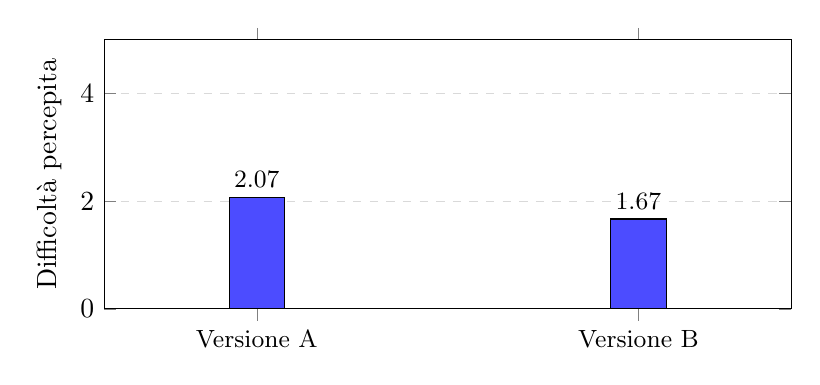
\begin{tikzpicture}
		\begin{axis}[
				ybar,
				bar width=20pt,
				width=0.85\textwidth,
				height=5cm,
				symbolic x coords={Versione A, Versione B},
				xtick=data,
				x tick label style={font=\small},
				ylabel={Difficoltà percepita},
				ymin=0, ymax=5,
				ymajorgrids=true,
				grid style={dashed, gray!30},
				enlarge x limits=0.4,
				nodes near coords,
				every node near coord/.style={font=\small, color=black},
			]
			\addplot+[
				ybar,
				fill=blue!70,
				draw=black
			] coordinates {
					(Versione A,2.07)
					(Versione B,1.67)
				};
		\end{axis}
	\end{tikzpicture}
	\caption{Confronto della difficoltà percepita tra Versione A e Versione B per C2.}
	\label{fig:6-c2-1}
\end{figure}

\begin{table}[H]
	\centering
	\footnotesize
	\renewcommand{\arraystretch}{1.2}
	\caption{Metriche prestazionali globali aggregate per il compito C2.}
	\label{tab:6-c2-1}
	\begin{tabular}{|>{\raggedright\arraybackslash}p{2.2cm}|>{\centering\arraybackslash}p{1.5cm}|>{\centering\arraybackslash}p{1.5cm}|>{\centering\arraybackslash}p{1.5cm}|>{\centering\arraybackslash}p{1.5cm}|>{\centering\arraybackslash}p{1.8cm}|>{\centering\arraybackslash}p{1.6cm}|}
		\hline
		\rowcolor{gray!30}
		\textbf{C2}           & \multicolumn{2}{c|}{\textbf{Versione A}} & \multicolumn{2}{c|}{\textbf{Versione B}} & \textbf{Variazione \%} & \textbf{Rilevanza}                                            \\ \hline
		\textit{Success Rate} & \multicolumn{2}{c|}{100,00\%}            & \multicolumn{2}{c|}{100,00\%}            & \textbf{Invariato}     &                                                               \\ \hline
		\rowcolor{gray!30}
		                      & \textbf{Media}                           & \textbf{DEV.ST}                          & \textbf{Media}         & \textbf{DEV.ST}    & \multicolumn{2}{c|}{}                    \\ \hline
		\textit{Errori}       & 1,07                                     & 1,03280                                  & 0,267                  & 0,45774            & \textbf{-75,00\%}     & \pvalue{0,00856} \\ \hline
		\textit{Tempo}        & 2.13.44                                  & 0,03596                                  & 2.00.08                & 0,01931            & \textbf{-10,17\%}     & \pvalue{0,20212} \\ \hline
		\textit{Click}        & 25,93                                    & 8,85169                                  & 13,33                  & 2,52605            & \textbf{-48,59\%}     & \pvalue{0,00007} \\ \hline
		\rowcolor{gray!30}
		                      & \multicolumn{2}{c|}{\textbf{Mediana}}    & \multicolumn{2}{c|}{\textbf{Mediana}}    & \multicolumn{2}{c|}{}                                                                  \\ \hline
		\textit{Difficoltà}   & \multicolumn{2}{c|}{2}                   & \multicolumn{2}{c|}{2}                   & \multicolumn{2}{c|}{}                                                                  \\ \hline
	\end{tabular}
\end{table}

La drastica diminuzione del numero medio di errori e dei click complessivi testimonia la maggiore linearità introdotta nella versione B. La riorganizzazione dell'interfaccia ha semplificato il processo di caricamento dei file e creazione delle cartelle, riducendo i passaggi superflui senza compromettere la rapidità dell'interazione.

\paragraph{Analisi qualitativa: commenti e osservazioni degli utenti}

I risultati quantitativi trovano riscontro nelle osservazioni raccolte durante le sessioni di test e nei commenti espressi dagli utenti. Per la versione originale (A), sono emerse criticità ricorrenti:

\begin{itemize}
	\item \textbf{Scarsa visibilità dei comandi e layout poco chiaro}: gli utenti hanno riportato difficoltà nell’individuare i controlli per il caricamento dei file e la creazione delle cartelle. Il posizionamento del comando di upload nella parte superiore dell’interfaccia è stato spesso percepito come poco intuitivo.

	\item \textbf{Problemi tecnici e perdita del contesto}: il flusso di caricamento è stato influenzato da un comportamento di refresh della pagina, che ha generato perdita temporanea del contesto operativo. In alcuni casi ciò ha portato alla mancata compilazione di campi obbligatori.

	\item \textbf{Carenze nella validazione e coerenza linguistica}: il sistema non forniva un adeguato supporto nella segnalazione degli errori in caso di campi incompleti. Inoltre, la presenza di etichette in lingua inglese in alcune componenti dell’interfaccia ha ridotto la coerenza linguistica complessiva.
\end{itemize}

Per la versione post-riprogettazione (B), i feedback indicano un miglioramento generale dell’esperienza, con alcune osservazioni residue:

\begin{itemize}
	\item \textbf{Criticità residue nella visibilità delle azioni}: nonostante i significativi miglioramenti riscontrati nelle metriche quantitative, l'operazione ha continuato a generare alcuni dubbi legati al posizionamento dei pulsanti e alla disposizione di determinati elementi dell'interfaccia. Alcuni utenti hanno segnalato come poco intuitiva la posizione iniziale della sidebar dedicata alla navigazione e alla gestione delle cartelle. È stato inoltre suggerito di rendere il pulsante per la creazione di una nuova cartella maggiormente visibile e accessibile, collocandolo in prossimità del pulsante di caricamento dei file. Un'ulteriore osservazione ha riguardato l'etichetta del pulsante utilizzato per il caricamento dei documenti: il termine ``Nuovo'' è stato ritenuto ambiguo poiché associato più facilmente alla creazione di un nuovo elemento (spesso interpretato come una cartella), mentre la dicitura ``Carica'' descriverebbe in modo più chiaro e immediato l'azione effettivamente eseguita.

	\item \textbf{Suggerimenti su flussi operativi alternativi}: è stata segnalata in più casi la mancanza di un flusso ibrido che consenta di caricare un file e creare contestualmente la cartella di destinazione, piuttosto che agire in due momenti separati.
\end{itemize}

\paragraph{Valutazione dell'effetto di apprendimento}

Analizzando i dati in base all'ordine di esecuzione (Tabella~\ref{tab:6-c2-2}), emergono dinamiche estremamente interessanti relative all'apprendimento e all'usabilità delle due interfacce. Nel gruppo che ha affrontato la sequenza A--B, il passaggio alla versione riprogettata si traduce in un miglioramento sistematico e robusto in tutte le metriche. Il tempo medio di completamento scende del 25,02\% (da 2:40.20 a 2:00.13), una contrazione solida e statisticamente rilevante. Registriamo inoltre variazioni sistematiche e non attribuibili al caso sia nella media degli errori, che cala dell'81,82\% (da 1,22 a 0,222), sia nel numero medio di click, ridotto del 48,56\% (da 27,00 a 13,89). Questi risultati indicano che l'esperienza maturata sulla prima interfaccia, unita ai miglioramenti strutturali della seconda, ha ottimizzato notevolmente l'interazione.

Nel gruppo B--A, il quadro si presenta differente. Si osserva un decremento del tempo medio di esecuzione, che tuttavia si qualifica come semplice andamento positivo ma non determinante sotto il profilo inferenziale. Di contro, gli utenti che passano dalla versione B alla versione originale (A) mostrano tendenze di peggioramento nelle altre prestazioni, caratterizzate da un incremento della media degli errori e da un aumento del numero medio di click. Sebbene queste variazioni rappresentino semplici tendenze descrittive (con il numero di click che si avvicina alla soglia di significatività), questo andamento suggerisce che la familiarizzazione con il compito non è bastata a compensare le inefficienze strutturali della vecchia interfaccia A. Gli utenti, pur conoscendo la sequenza di azioni necessarie, sono stati costretti a compiere più errori e click per completare il caricamento del file.

\begin{table}[H]
	\centering
	\footnotesize
	\renewcommand{\arraystretch}{1.2}
	\caption{Confronto delle metriche prestazionali in funzione dell'ordine di esecuzione per il compito C2.}
	\label{tab:6-c2-2}
	\begin{tabular}{|>{\raggedright\arraybackslash}p{2.2cm}|>{\centering\arraybackslash}p{1.0cm}|>{\centering\arraybackslash}p{1.0cm}|>{\centering\arraybackslash}p{1.8cm}|>{\centering\arraybackslash}p{1.6cm}|>{\centering\arraybackslash}p{1.0cm}|>{\centering\arraybackslash}p{1.0cm}|>{\centering\arraybackslash}p{1.8cm}|>{\centering\arraybackslash}p{1.6cm}|}
		\hline
		\rowcolor{gray!30}
		\textbf{Metrica}              & \multicolumn{4}{c|}{\textbf{Ordine A--B}} & \multicolumn{4}{c|}{\textbf{Ordine B--A}}                                                                                                                       \\ \cline{2-9}
		\rowcolor{gray!30}
		                              & \textbf{A}                                & \textbf{B}                                & \textbf{Variazione \%} & \textbf{Rilevanza} & \textbf{B} & \textbf{A} & \textbf{Variazione \%} & \textbf{Rilevanza} \\ \hline
		\textit{Tempo (Media)}        & 2.40.20                                   & 2.00.13                                   & \textbf{-25,02\%}      & \pvalue{0,01312}   & 2.00.00    & 1.33.50    & \textbf{-21,81\%}      & \pvalue{0,09526}   \\ \hline
		\textit{Errori (Media)}       & 1,22                                      & 0,222                                     & \textbf{-81,82\%}      & \pvalue{0,00852}   & 0,333      & 0,83       & \textbf{150,00\%}      & \pvalue{0,29556}   \\ \hline
		\textit{Click (Media)}        & 27,00                                     & 13,89                                     & \textbf{-48,56\%}      & \pvalue{0,00030}   & 12,50      & 24,33      & \textbf{94,67\%}       & \pvalue{0,05806}   \\ \hline
		\textit{Difficoltà (Mediana)} & 1                                         & 1                                         &                        & \pvalue{}          & 2          & 3,5        &                        & \pvalue{}          \\ \hline
	\end{tabular}
\end{table}

Questa asimmetria è confermata e resa visibile dall'analisi della difficoltà percepita (Figura~\ref{fig:6-c2-2}). Nel gruppo con ordine B--A, si rileva un netto incremento della fatica percepita nel passaggio alla vecchia interfaccia: la mediana sale da 2 a 3,5, con un punteggio medio che compie un salto vistoso attestandosi a 3,00 per la Versione A. Questo incremento testimonia come l'abitudine alla fluidità della versione B renda ancora più frustranti le barriere all'usabilità della versione originale. Al contrario, nel gruppo A--B la mediana si attesta a 1 in entrambe le condizioni e i punteggi medi rimangono molto vicini (1,44 per la versione A e 1,56 per la versione B); in questa sequenza, lo sforzo iniziale speso per comprendere l'interfaccia originale sembra aver appiattito la percezione di difficoltà successiva, dove piccoli dettagli della versione B (come l'ambiguità del pulsante ``Nuovo'') hanno bilanciato i benefici strutturali della riprogettazione.

\begin{figure}[H]
	\centering
	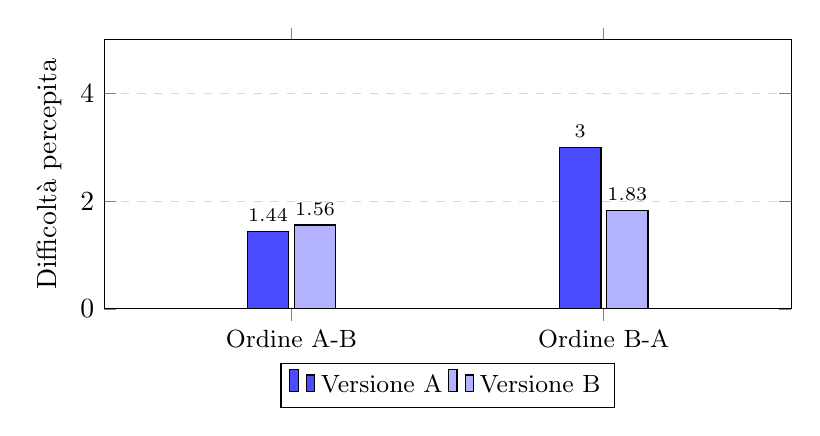
\begin{tikzpicture}
		\begin{axis}[
				ybar,
				bar width=15pt,
				width=0.85\textwidth,
				height=5cm,
				symbolic x coords={Ordine A-B, Ordine B-A},
				xtick=data,
				x tick label style={font=\small},
				ylabel={Difficoltà percepita},
				ymin=0, ymax=5,
				ymajorgrids=true,
				grid style={dashed, gray!30},
				enlarge x limits=0.6,
				legend style={at={(0.5,-0.2)}, anchor=north, legend columns=-1, font=\small},
				nodes near coords,
				every node near coord/.append style={font=\scriptsize, color=black},
			]
			\addplot+[
				fill=blue!70,
				draw=black
			] coordinates {
					(Ordine A-B,1.44)
					(Ordine B-A,3.00)
				};
			\addplot+[
				fill=blue!30,
				draw=black
			] coordinates {
					(Ordine A-B,1.56)
					(Ordine B-A,1.83)
				};
			\legend{Versione A, Versione B}
		\end{axis}
	\end{tikzpicture}
	\caption{Confronto della difficoltà percepita tra Versione A e Versione B per C2 in base all'ordine di esecuzione.}
	\label{fig:6-c2-2}
\end{figure}

\subsubsection{Compito C3: Pianificare un esame}

Il compito C3 richiedeva all'utente di pianificare un nuovo esame denominato "Architettura" con data 22/09/2026, associando un'attività specifica ("Riassumere il primo capitolo") e collegando al piano di studio il documento "Appunti\_Lezione.pdf" caricato nel compito precedente. L'obiettivo era valutare l'usabilità del sistema di organizzazione dello studio, con particolare attenzione ai percorsi di navigazione verso la sezione dedicata agli esami e all'intuitività dell'interfaccia per la gestione dei task e dei materiali allegati.

\paragraph{Analisi delle prestazioni generali}

Come si può notare dai dati aggregati per il compito C3 (Tabella~\ref{tab:6-c3-1}), il tasso di completamento (Success Rate) si è attestato al 100,00\% per entrambe le versioni del sistema. La versione post-riprogettazione (B) evidenzia miglioramenti su tutte le metriche considerate: la media degli errori si riduce del 57,14\% (da 0,93 a 0,40) e la mediana dei click diminuisce del 34,78\% (da 23 a 15). Si osserva inoltre una riduzione del 21,05\% nel tempo mediano di esecuzione e un calo del 29,27\% nella difficoltà percepita dagli utenti.

\begin{figure}[H]
	\centering
	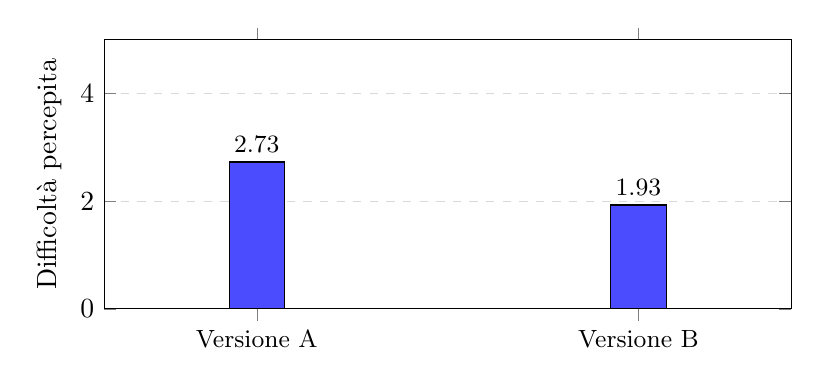
\begin{tikzpicture}
		\begin{axis}[
				ybar,
				bar width=20pt,
				width=0.85\textwidth,
				height=5cm,
				symbolic x coords={Versione A, Versione B},
				xtick=data,
				x tick label style={font=\small},
				ylabel={Difficoltà percepita},
				ymin=0, ymax=5,
				ymajorgrids=true,
				grid style={dashed, gray!30},
				enlarge x limits=0.4,
				nodes near coords,
				every node near coord/.style={font=\small, color=black},
			]
			\addplot+[
				ybar,
				fill=blue!70,
				draw=black
			] coordinates {
					(Versione A,2.73)
					(Versione B,1.93)
				};
		\end{axis}
	\end{tikzpicture}
	\caption{Confronto della difficoltà percepita tra Versione A e Versione B per C3.}
	\label{fig:6-c3-1}
\end{figure}

\begin{table}[H]
	\centering
	\footnotesize
	\renewcommand{\arraystretch}{1.2}
	\caption{Metriche prestazionali globali aggregate per il compito C3.}
	\label{tab:6-c3-1}
	\begin{tabular}{|>{\raggedright\arraybackslash}p{2.2cm}|>{\centering\arraybackslash}p{1.5cm}|>{\centering\arraybackslash}p{1.5cm}|>{\centering\arraybackslash}p{1.5cm}|>{\centering\arraybackslash}p{1.5cm}|>{\centering\arraybackslash}p{1.8cm}|>{\centering\arraybackslash}p{1.6cm}|}
		\hline
		\rowcolor{gray!30}
		\textbf{C3}           & \multicolumn{2}{c|}{\textbf{Versione A}} & \multicolumn{2}{c|}{\textbf{Versione B}} & \textbf{Variazione \%} & \textbf{Rilevanza}                                            \\ \hline
		\textit{Success Rate} & \multicolumn{2}{c|}{100,00\%}            & \multicolumn{2}{c|}{100,00\%}            & \textbf{Invariato}     &                                                               \\ \hline
		\rowcolor{gray!30}
		                      & \textbf{Media}                           & \textbf{DEV.ST}                          & \textbf{Media}         & \textbf{DEV.ST}    & \multicolumn{2}{c|}{}                    \\ \hline
		\textit{Errori}       & 0,93                                     & 1,22280                                  & 0,400                  & 0,73679            & \textbf{-57,14\%}     & \pvalue{0,13496} \\ \hline
		\textit{Tempo}        & 2.15.28                                  & 0,04102                                  & 1.43.08                & 0,02792            & \textbf{-23,87\%}     & \pvalue{0,05534} \\ \hline
		\textit{Click}        & 24,47                                    & 6,77038                                  & 14,20                  & 3,14416            & \textbf{-41,96\%}     & \pvalue{0,00014} \\ \hline
		\rowcolor{gray!30}
		                      & \multicolumn{2}{c|}{\textbf{Mediana}}    & \multicolumn{2}{c|}{\textbf{Mediana}}    & \multicolumn{2}{c|}{}                                                                  \\ \hline
		\textit{Difficoltà}   & \multicolumn{2}{c|}{3}                   & \multicolumn{2}{c|}{2}                   & \multicolumn{2}{c|}{}                                                                  \\ \hline
	\end{tabular}
\end{table}

La riduzione dei tempi, dei click e del tasso di errore indica che il redesign ha migliorato la navigabilità del sistema e la visibilità della sezione dedicata agli esami. La riorganizzazione dell’interfaccia e la semplificazione dei percorsi di accesso hanno consentito una maggiore immediatezza nell’esecuzione del compito e una riduzione del carico cognitivo.

\paragraph{Analisi qualitativa: commenti e osservazioni degli utenti}

I risultati quantitativi trovano riscontro nelle osservazioni qualitative e nei commenti raccolti. Per la versione originale (A), sono emerse criticità ricorrenti:

\begin{itemize}
	\item \textbf{Disorientamento e terminologia poco chiara}: la navigazione è risultata difficoltosa a causa dell’uso dell’etichetta "StudyFlow AI" per la sezione dedicata agli esami. Tale denominazione è stata frequentemente percepita come poco rappresentativa della funzionalità, generando incertezza nell’individuazione della sezione corretta.

	\item \textbf{Architettura dell’informazione poco coerente}: l’interfaccia è stata descritta come poco lineare, con molteplici modi per eseguire le stesse operazioni. In particolare, la necessità di passare dalla dashboard principale per creare un nuovo esame è stata percepita come un passaggio non necessario, portando in alcuni casi all’utilizzo della dashboard come punto di accesso alternativo.

	\item \textbf{Scarsa visibilità dei controlli}: anche la funzione di associazione dei materiali di studio ha presentato difficoltà di individuazione, risultando poco evidente e non immediatamente accessibile.
\end{itemize}

Per la versione post-riprogettazione (B), i risultati indicano un miglioramento generale dell’esperienza, pur con alcuni margini residui di ottimizzazione:

\begin{itemize}
	\item \textbf{Maggiore chiarezza della navigazione}: l’interfaccia è stata percepita come più semplice e coerente. L’accesso diretto alla sezione "Esami" ha ridotto le difficoltà di individuazione della funzionalità rispetto alla versione precedente.

	\item \textbf{Affinamenti necessari nei micro-flussi}: nonostante il miglioramento complessivo, alcuni utenti hanno segnalato incertezze nella gestione delle attività secondarie. In particolare, l’uso di un’icona a freccia per la rimozione di un task è stato talvolta ritenuto poco intuitivo.
\end{itemize}

\paragraph{Valutazione dell'effetto di apprendimento}

Analizzando i dati in base all'ordine di esecuzione (Tabella~\ref{tab:6-c3-2}) risulta chiaro che, in questo caso, l'esperienza pregressa dell'utente conta meno rispetto alla struttura dell'interfaccia.

Nel gruppo A--B, il tempo mediano di esecuzione passa da 1:53 (versione A) a 1:27 (versione B), con una riduzione del 23,01\%.

Nel gruppo B--A, gli utenti completano inizialmente il compito sulla versione B in 1:46,5, mentre nella successiva interazione con la versione A il tempo mediano aumenta fino a 2:02. Questo risultato suggerisce che l’esperienza maturata con la versione più ottimizzata non si trasferisce in modo efficace alla versione originale, le cui criticità strutturali continuano a incidere in maniera significativa sulle prestazioni, indipendentemente dalla familiarità con il task.

\begin{table}[H]
	\centering
	\footnotesize
	\renewcommand{\arraystretch}{1.2}
	\caption{Confronto delle metriche prestazionali in funzione dell'ordine di esecuzione per il compito C3.}
	\label{tab:6-c3-2}
	\begin{tabular}{|>{\raggedright\arraybackslash}p{2.2cm}|>{\centering\arraybackslash}p{1.0cm}|>{\centering\arraybackslash}p{1.0cm}|>{\centering\arraybackslash}p{1.8cm}|>{\centering\arraybackslash}p{1.6cm}|>{\centering\arraybackslash}p{1.0cm}|>{\centering\arraybackslash}p{1.0cm}|>{\centering\arraybackslash}p{1.8cm}|>{\centering\arraybackslash}p{1.6cm}|}
		\hline
		\rowcolor{gray!30}
		\textbf{Metrica}              & \multicolumn{4}{c|}{\textbf{Ordine A--B}}                                                 & \multicolumn{4}{c|}{\textbf{Ordine B--A}}                                                 \\ \cline{2-9} 
		\rowcolor{gray!30}
		                              & \textbf{A}          & \textbf{B}          & \textbf{Variazione \%} & \textbf{Rilevanza}        & \textbf{B}          & \textbf{A}          & \textbf{Variazione \%} & \textbf{Rilevanza}        \\ \hline
		\textit{Tempo (Media)}        & 2.14.20             & 1.31.20             & \textbf{-32,01\%}      & \pvalue{0,02105}          & 2.00.50             & 2.17.10             & \textbf{13,52\%}       & \pvalue{0,40930}          \\ \hline
		\textit{Errori (Media)}       & 1,22                & 0,667               & \textbf{-45,45\%}      & \pvalue{0,21446}          & 0,000               & 0,50                & \textbf{Invariato}     & \pvalue{0,20311}          \\ \hline
		\textit{Click (Media)}        & 22,22               & 14,89               & \textbf{-33,00\%}      & \pvalue{0,00442}          & 13,17               & 27,83               & \textbf{111,39\%}      & \pvalue{0,00755}          \\ \hline
		\textit{Difficoltà (Mediana)} & 2                   & 1                   &                        & \pvalue{}                 & 2                   & 3,5                 &                        & \pvalue{}                 \\ \hline
	\end{tabular}
\end{table}

Le stesse criticità si riflettono sulle valutazioni di difficoltà riassunte nella Figura~\ref{fig:6-c3-2}. Nel gruppo B–A si nota lo stacco più evidente: gli utenti che iniziano con la Versione B assegnano un punteggio di 2,00, ma al successivo passaggio alla versione originale (A) la difficoltà percepita aumenta sensibilmente, raggiungendo un valore di 3,50. Questo valore dimostra che, dopo aver utilizzato la versione chiara, l'impatto con l'etichetta "StudyFlow AI" e i passaggi forzati dalla dashboard della versione A diventa ancora più frustrante. Nel gruppo A--B, invece, la variazione è stata inferiore alle aspettative (da 2,22 a 1,89), simbolo che aver affrontato prima la versione complicata ha aiutato gli utenti a capire come funzionava la piattaforma, rendendo poi il passaggio alla versione B più morbido, anche se i piccoli difetti rimasti (come la freccia poco intuitiva per cancellare i task) hanno impedito al punteggio di scendere ancora di più.

\begin{figure}[H]
	\centering
	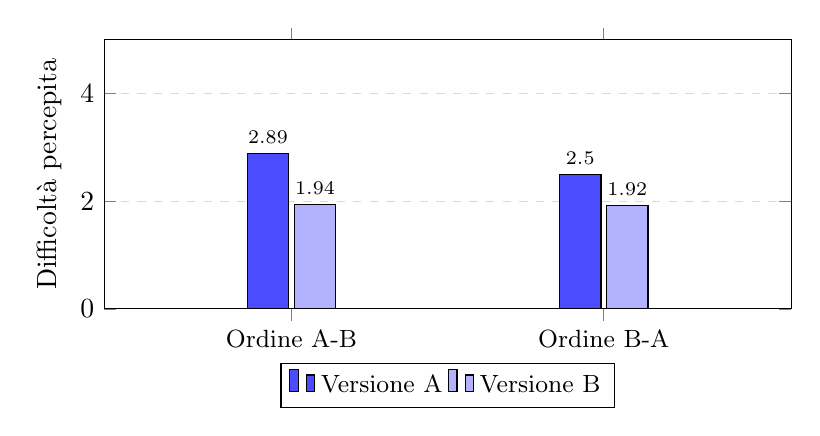
\begin{tikzpicture}
		\begin{axis}[
				ybar,
				bar width=15pt,
				width=0.85\textwidth,
				height=5cm,
				symbolic x coords={Ordine A-B, Ordine B-A},
				xtick=data,
				x tick label style={font=\small},
				ylabel={Difficoltà percepita},
				ymin=0, ymax=5,
				ymajorgrids=true,
				grid style={dashed, gray!30},
				enlarge x limits=0.6,
				legend style={at={(0.5,-0.2)}, anchor=north, legend columns=-1, font=\small},
				nodes near coords,
				every node near coord/.append style={font=\scriptsize, color=black},
			]
			\addplot+[
				fill=blue!70,
				draw=black
			] coordinates {
					(Ordine A-B,2.89)
					(Ordine B-A,2.50)
				};
			\addplot+[
				fill=blue!30,
				draw=black
			] coordinates {
					(Ordine A-B,1.94)
					(Ordine B-A,1.92)
				};
			\legend{Versione A, Versione B}
		\end{axis}
	\end{tikzpicture}
	\caption{Confronto della difficoltà percepita tra Versione A e Versione B per C3 in base all'ordine di esecuzione.}
	\label{fig:6-c3-2}
\end{figure}

